\begin{center}
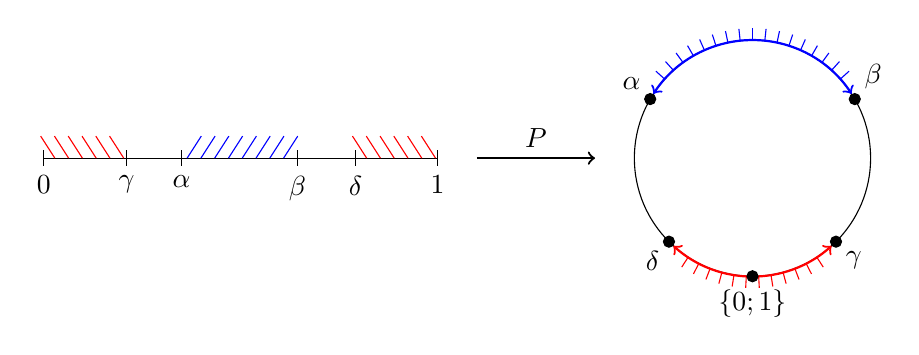
\begin{tikzpicture}
    \def\x{5}
    \def\tick{0.1}
    \def\gam{0.31*\x}
    \def\alp{0.35*\x}
    \def\bet{0.65*\x}
    \def\delt{0.8*\x}
    \def\radius{1.5}
    

    % shorter hatch length
    \def\h{0.15}
    
    % hatch style
    \def\vx{0.18}
    \def\vy{0.28}

% --------------------
% Number line
% --------------------
\draw (0,0) -- (\x,0);

% --------------------
% BLUE interval (alpha=1.75, beta=3.25)
% --------------------
\draw[blue] (\alp+0.02*3.5,0) -- ++(\vx,\vy);
\draw[blue] (\alp+0.07*3.5,0) -- ++(\vx,\vy);
\draw[blue] (\alp+0.12*3.5,0) -- ++(\vx,\vy);
\draw[blue] (\alp+0.17*3.5,0) -- ++(\vx,\vy);
\draw[blue] (\alp+0.22*3.5,0) -- ++(\vx,\vy);
\draw[blue] (\alp+0.27*3.5,0) -- ++(\vx,\vy);
\draw[blue] (\alp+0.32*3.5,0) -- ++(\vx,\vy);
\draw[blue] (\alp+0.37*3.5,0) -- ++(\vx,\vy);

% --------------------
% RED interval [0, gamma=1]
% --------------------
\draw[red] (0.14,0) -- ++(-\vx,\vy);
\draw[red] (0.14+0.05*3.5,0) -- ++(-\vx,\vy);
\draw[red] (0.14+0.10*3.5,0) -- ++(-\vx,\vy);
\draw[red] (0.14+0.15*3.5,0) -- ++(-\vx,\vy);
\draw[red] (0.14+0.20*3.5,0) -- ++(-\vx,\vy);
\draw[red] (0.14+0.25*3.5,0) -- ++(-\vx,\vy);

% --------------------
% RED interval [delta=4, 1]
% --------------------
\draw[red] (4.1,0) -- ++(-\vx,\vy);
\draw[red] (4.1+0.05*3.5,0) -- ++(-\vx,\vy);
\draw[red] (4.1+0.10*3.5,0) -- ++(-\vx,\vy);
\draw[red] (4.1+0.15*3.5,0) -- ++(-\vx,\vy);
\draw[red] (4.1+0.20*3.5,0) -- ++(-\vx,\vy);
\draw[red] (4.1+0.25*3.5,0) -- ++(-\vx,\vy);

% --------------------
% ticks and labels
% --------------------
\draw (0,\tick) -- ++(0,-2*\tick) node[below] {$0$};
\draw (1.05,\tick) -- ++(0,-2*\tick) node[below] {$\gamma$};
\draw (1.75,\tick) -- ++(0,-2*\tick) node[below] {$\alpha$};
\draw (3.22,\tick) -- ++(0,-2*\tick) node[below] {$\beta$};
\draw (4-0.04,\tick) -- ++(0,-2*\tick) node[below] {$\delta$};
\draw (5,\tick) -- ++(0,-2*\tick) node[below] {$1$};



    % --------------------
    % Circle
    % --------------------
    \draw (\x+4,0) circle (\radius);
    
    \draw[->, thick] (\x+0.5,0) -- (\x+2,0) node[midway, above] {$P$};
    
    % Points
    \filldraw (\x+4,0) ++(30:\radius) circle (2pt) node[above right] {$\beta$};
    \filldraw (\x+4,0) ++(150:\radius) circle (2pt) node[above left] {$\alpha$};
    \filldraw (\x+4,0) ++(225:\radius) circle (2pt) node[below left] {$\delta$};
    \filldraw (\x+4,0) ++(315:\radius) circle (2pt) node[below right] {$\gamma$};

    % --------------------
    % Blue arc
    % --------------------
    \draw[thick, blue, <->] (\x+4,0) ++(33:\radius) arc (33:147:\radius);

    % moderate density, outward only
    \foreach \t in {42,48,...,143} {
        \draw[blue]
        ({\x+4 + \radius*cos(\t)}, {\radius*sin(\t)})
        -- ({\x+4 + (\radius+\h)*cos(\t)}, {(\radius+\h)*sin(\t)});
    }

    % --------------------
    % Red arc
    % --------------------
    \draw[thick, red, <->] (\x+4,0) ++(228:\radius) arc (228:312:\radius);

    \foreach \t in {237,243,...,304} {
        \draw[red]
        ({\x+4 + \radius*cos(\t)}, {\radius*sin(\t)})
        -- ({\x+4 + (\radius+\h)*cos(\t)}, {(\radius+\h)*sin(\t)});
    }

    % Bottom point
    \filldraw (\x+4,-1.5) circle (2pt) node[below,yshift=-1.4] {$\{0;1\}$};

\end{tikzpicture}
\end{center}